\subsection{Running-Time Analysis}

\subsubsection{Theoretical Analysis}

Let $n$ be the number of candidate windows. Sorting by
finishing time with the C++ standard library takes
$O(n\log n)$ comparisons \cite{cppreferenceSort}. The
selection loop then examines each window once with an
$O(1)$ compatibility check, taking $O(n)$ time. Since
sorting dominates,

\[
T(n) = O(n\log n) + O(n) = \boxed{O(n\log n)}.
\]

\subsubsection{Experimental Verification}

The algorithm was implemented in C++ and run on
randomly generated windows for seven input sizes from
1,000 to 200,000. Each size was run 10 times and the
median time recorded (Table~\ref{tab:greedy-runtime}),
using the \texttt{chrono} steady clock, excluding input
generation from the timed region, and compiling with
\texttt{-O2}.

\begin{table}[htbp]
\centering
\caption{Greedy Running-Time Results}
\label{tab:greedy-runtime}
\footnotesize
\begin{tabular}{|r|r|}
\hline
Input Size ($n$) & Median Time (ms) \\
\hline
1,000 & 0.03560 \\
5,000 & 0.19195 \\
10,000 & 0.43350 \\
25,000 & 1.10480 \\
50,000 & 2.36325 \\
100,000 & 4.75960 \\
200,000 & 10.90790 \\
\hline
\end{tabular}
\end{table}

Figure~\ref{fig:greedy-runtime} compares the measured
times with a scaled $O(n\log n)$ curve. The measurements
follow the theoretical growth closely; individual
deviations are attributable to system activity and
hardware effects.

\begin{figure}[htbp]
\centering
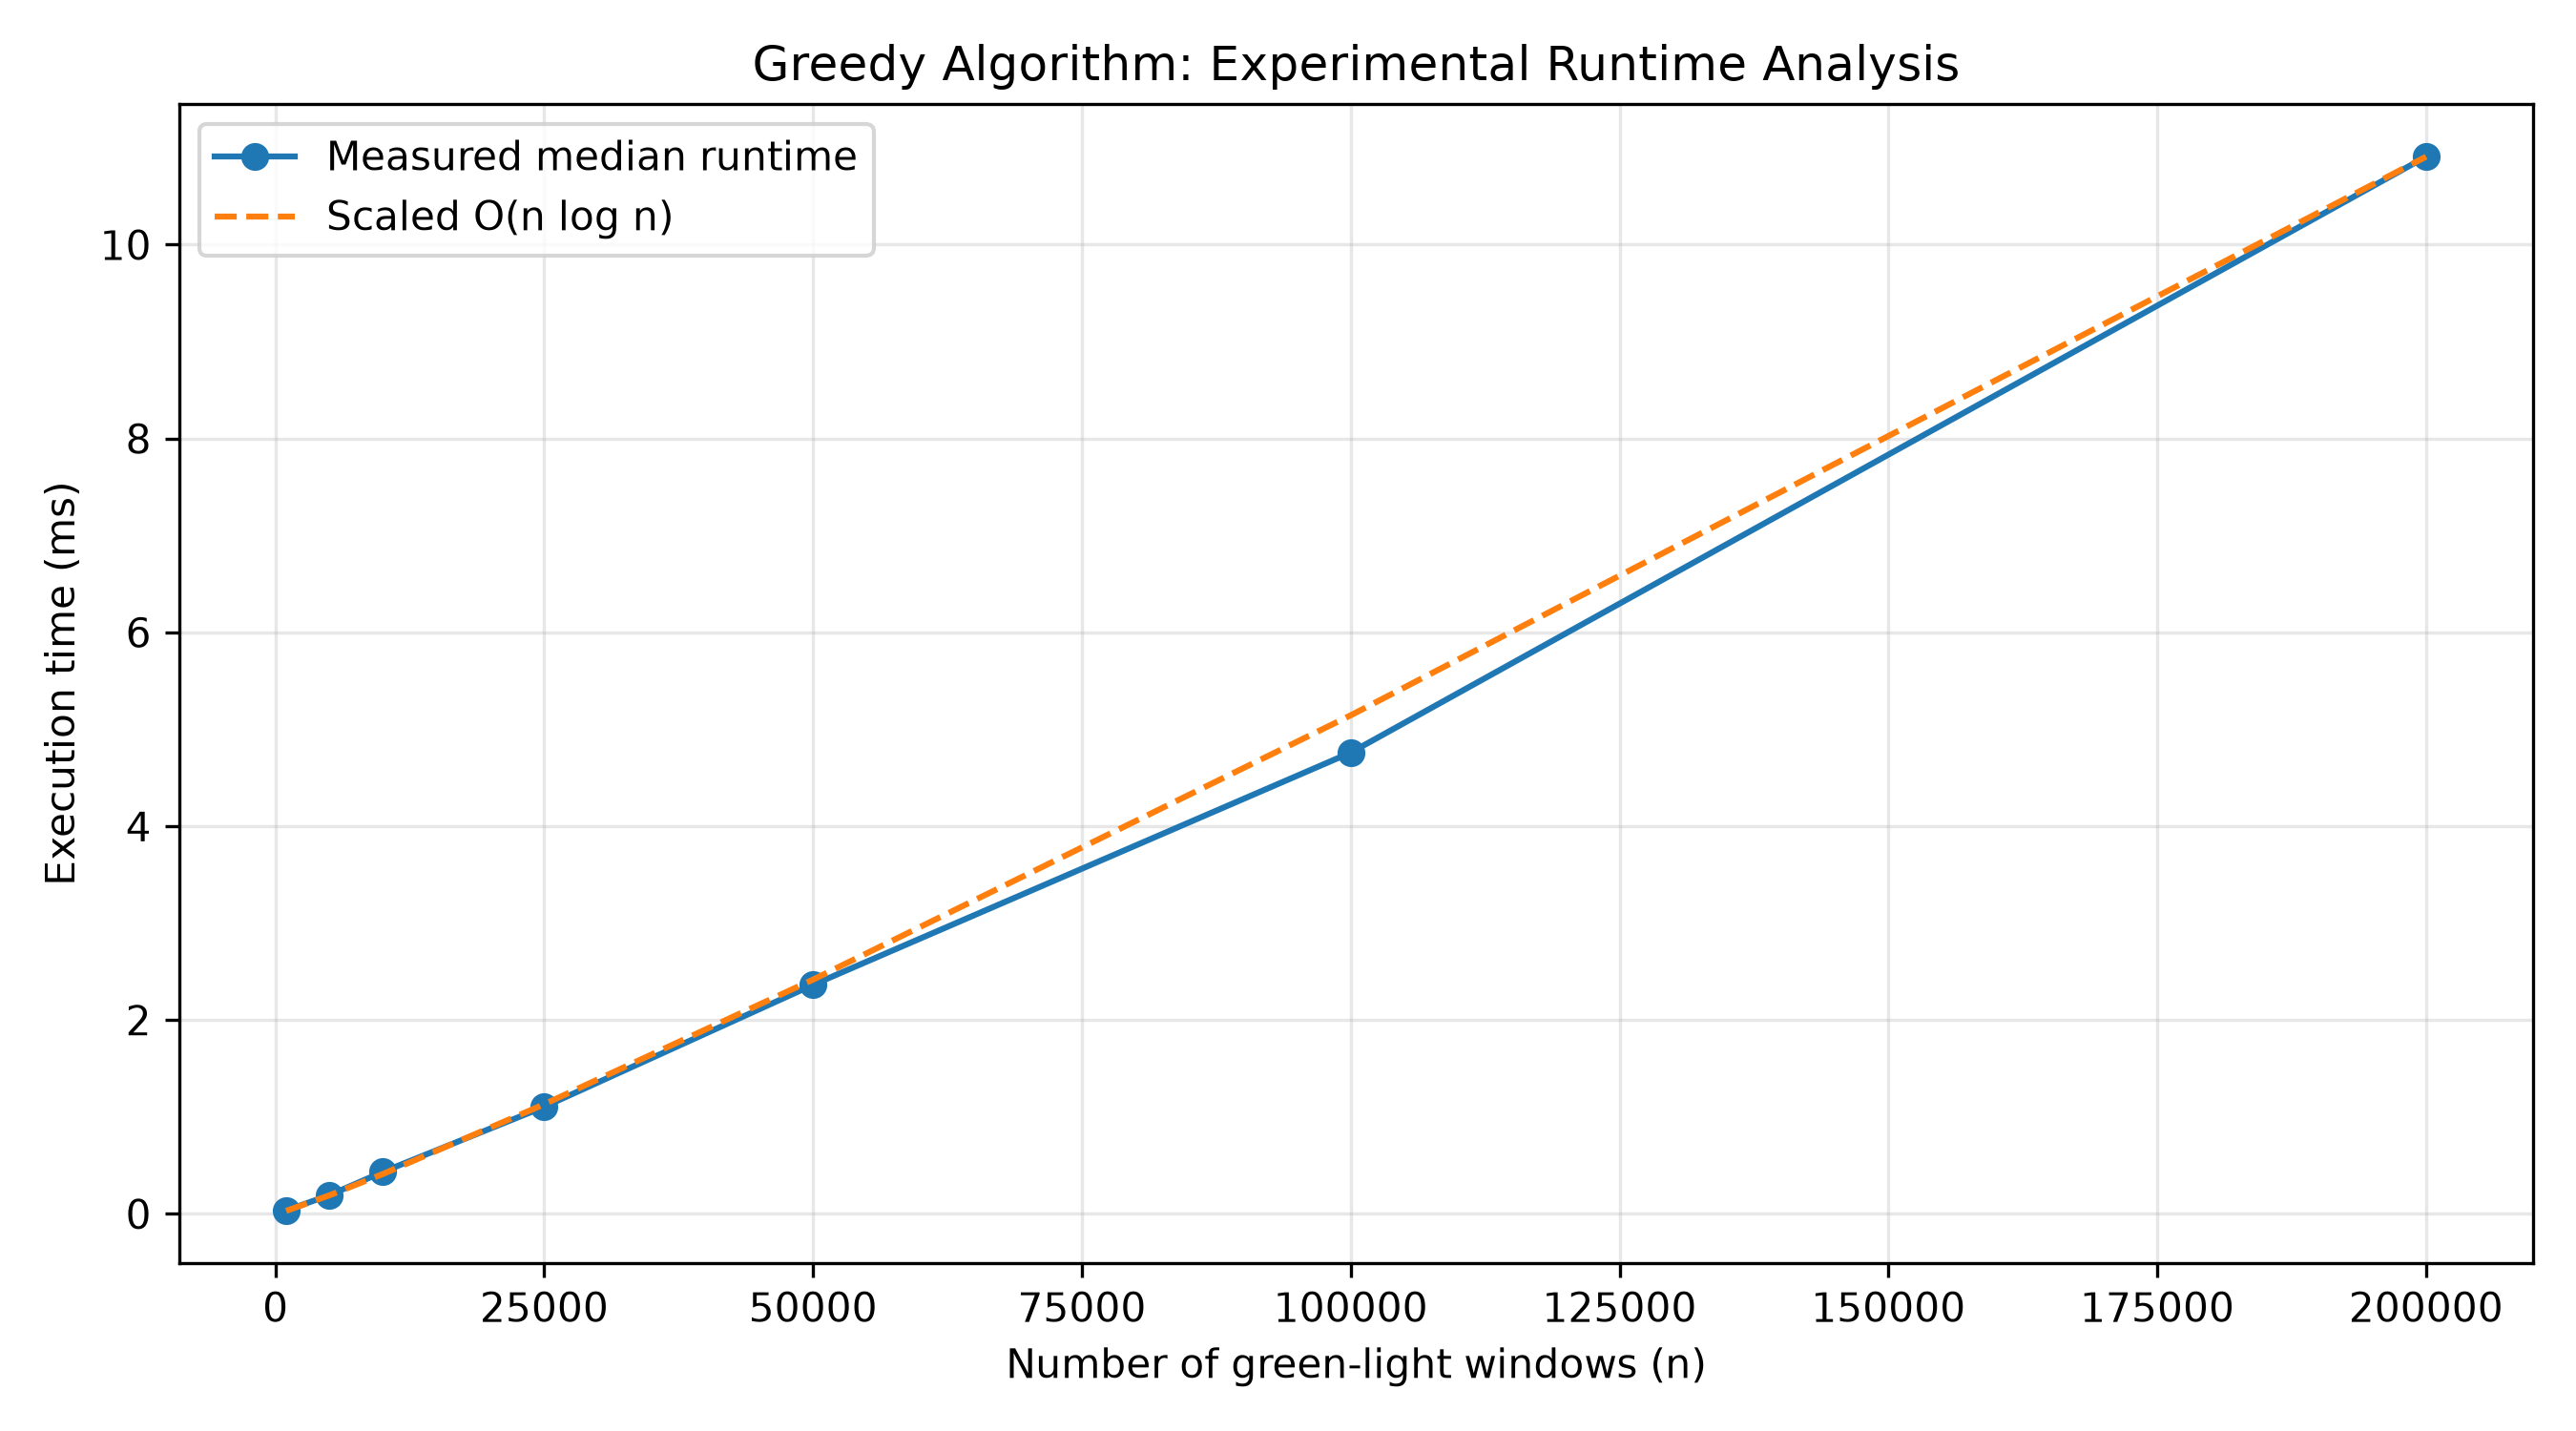
\includegraphics[width=0.9\linewidth]{runtime_graph.png}
\caption{Greedy algorithm: measured median time vs.\
scaled $O(n\log n)$ growth.}
\label{fig:greedy-runtime}
\end{figure}
